\section{\LARGE{Amplificazione RealTime PCR. Estrazione proteine totali}}

\vspace{0.6cm}

\subsection{Sommario}

\subsubsection{Scopo}

In questa esperienza vediamo due procedimenti:
\begin{itemize}
  \item Amplificazione di un cDNA tramite la PCR real time.
  \item L'estrazione delle proteine e la loro quantificazione al Qubit 3.
\end{itemize}

\subsubsection{Cenni teorici}

La PCR real time è una particolare PCR che ci permette di amplificare e
contemporaneamente quantificare il DNA in tempo reale osservando la fluorescenza
ad ogni iterazione.
%Paragonando due campioni diversi \`e possibile stabilire il rapporto tra le quantit\`a
%iniziali della sostanza.
Per rendere il campione fluorescente si utilizza una sonda composta da un colorante
fluorescente (Responser) e da un Quencer che assorbe l'energia della fluorescenza.
La sonda si lega tra i due primer (forward e reverse) del gene.
Quando la sonda viene degradata (dall'attivita' esonucleasica della TAQ-polimerasi)
il Quencer e il Responser si separano. In questo modo il Responser e' libero di emettere
fluorescenza che risulta visibile e misurabile.

\subsubsection{Strumenti e materiali utilizzati}

\begin{itemize}
\item Guanti in lattice
\item Provette Eppendorf (1.5ml)
\item Assay tube (500$\mu$l)
\item Micropipette (100-1000  e 2-200 $\mu$l)
\item Qubit 3 (per quantificare le proteine)
\end{itemize}

\subsubsection{Soluzioni utilizzate}
\begin{itemize}
\item cDNA
\item Pellet cellulare per l'estrazione delle proteine
\item RIPA buffer (soluzione tampone utilizzata per l'estrazione di proteine da cellule
di mammifero)
\item Working solution
\end{itemize}

\subsection{Procedimento}

\subsubsection{Amplificazione RealTime PCR}
\begin{itemize}
\item Prendere il cDNA dall'esperienza precedente
\item Utilizzare questa quantit\`a di reagenti per un volume finale di 40$\mu$l diviso in
due pozzetti da 20$\mu$l: \\
\begin{tabular}{c c c c}
\hline
Reagente & Concentrazione & $\mu$l/pozzetto & $\mu$l 2 pozzetti \\
\hline
MasterMix & 2X & 10$\mu$l & 20$\mu$l \\
Sonda TaqMal & 20X & 1$\mu$l & 2$\mu$l \\
H$_2$O & 1X & 7$\mu$l & 14$\mu$l \\
cDNA & 1X & 2$\mu$l & 4$\mu$l \\
\end{tabular}
\item Aliquotare ogni reagente in un'eppendorf da 1,5ml.
\item Spostare ogni reazione nei pozzetti (appoggiarsi al bordo per essere pi\`u precisi)
\item Sigillare con l'adesivo ottico
\item Centrifugare brevemente
\item Avviare la reazione di amplificazione \\
Questi sono i parametri del termociclatore:\\
\begin{tabular}{c c c c c}
\hline
Parametro & Incubazione UNG & Attivazione polimerasi &
\multicolumn{2}{c}{PCR (40 cicli)} \\
\hline
& Hold & Hold & Denaturazione & Annealing/estensione \\
\hline
Temperatura & 50C & 95C & 95C & 60C \\
\hline
Tempo (mm:ss) & 02:00 & 10:00 & 00:15 & 01:00 \\
\end{tabular}
\item Attendere il completamento ed analizzare i dati raccolti
\end{itemize}

\subsubsection{Estrazione delle proteine}
\begin{itemize}
\item Risospendere il pellet cellulare in 100ul di RIPA Buffer addizionato
di inibitori di proteasi con la diluizione: \\
\begin{tabular}{c c c}
Reagente & Concentrazione & Quantit\`a \\
RIPA buffer & 1X & 96ul \\
Inibitori & 25X & 4ul \\
& & TOT = 100$\mu$l \\
\end{tabular}
Il buffer di lisi serve a rompere le cellule.

\item Incubare per 45' in ghiaccio
\item Centrifugare per 40'' a 4°C
\item Prelevare il surnatante (contenente le proteine) in una nuova eppendorf
\item Conservare in ghiaccio
\end{itemize}

\subsubsection{Quantificazione proteine con Qubit 3}
\begin{itemize}
\item Preparare la Working Solution, che servir\`a sia per la taratura dello strumento
che per la misurazione della quantit\`a di proteine. Nel nostro caso lo strumento era
gi\`a stato tarato, quindi dalla tabella escludiamo le 3 dosi per la taratura.

\begin{tabular}{c c c}
Reagente & Quantit\`a 1 dose & Quantit\`a 10 dosi \\
Qubit protein reagent & 1ul & 10ul \\
Qubit protein buffer & 199ul & 1990ul \\
 & TOT = 200ul & TOT = 200ul \\
\end{tabular}

\item Aliquotare 190$\mu$l di Working Solution in un AsseyTube da 500$\mu$l
\item Aggiungere 10$\mu$l di proteine, invertire il tubo 10 volte e centrifugare brevemente
\item Lasciare la miscela al buio per 15'
\item Leggere l'emissione del fluoroforo

\end{itemize}

\begin{figure}[H]

	\centering
	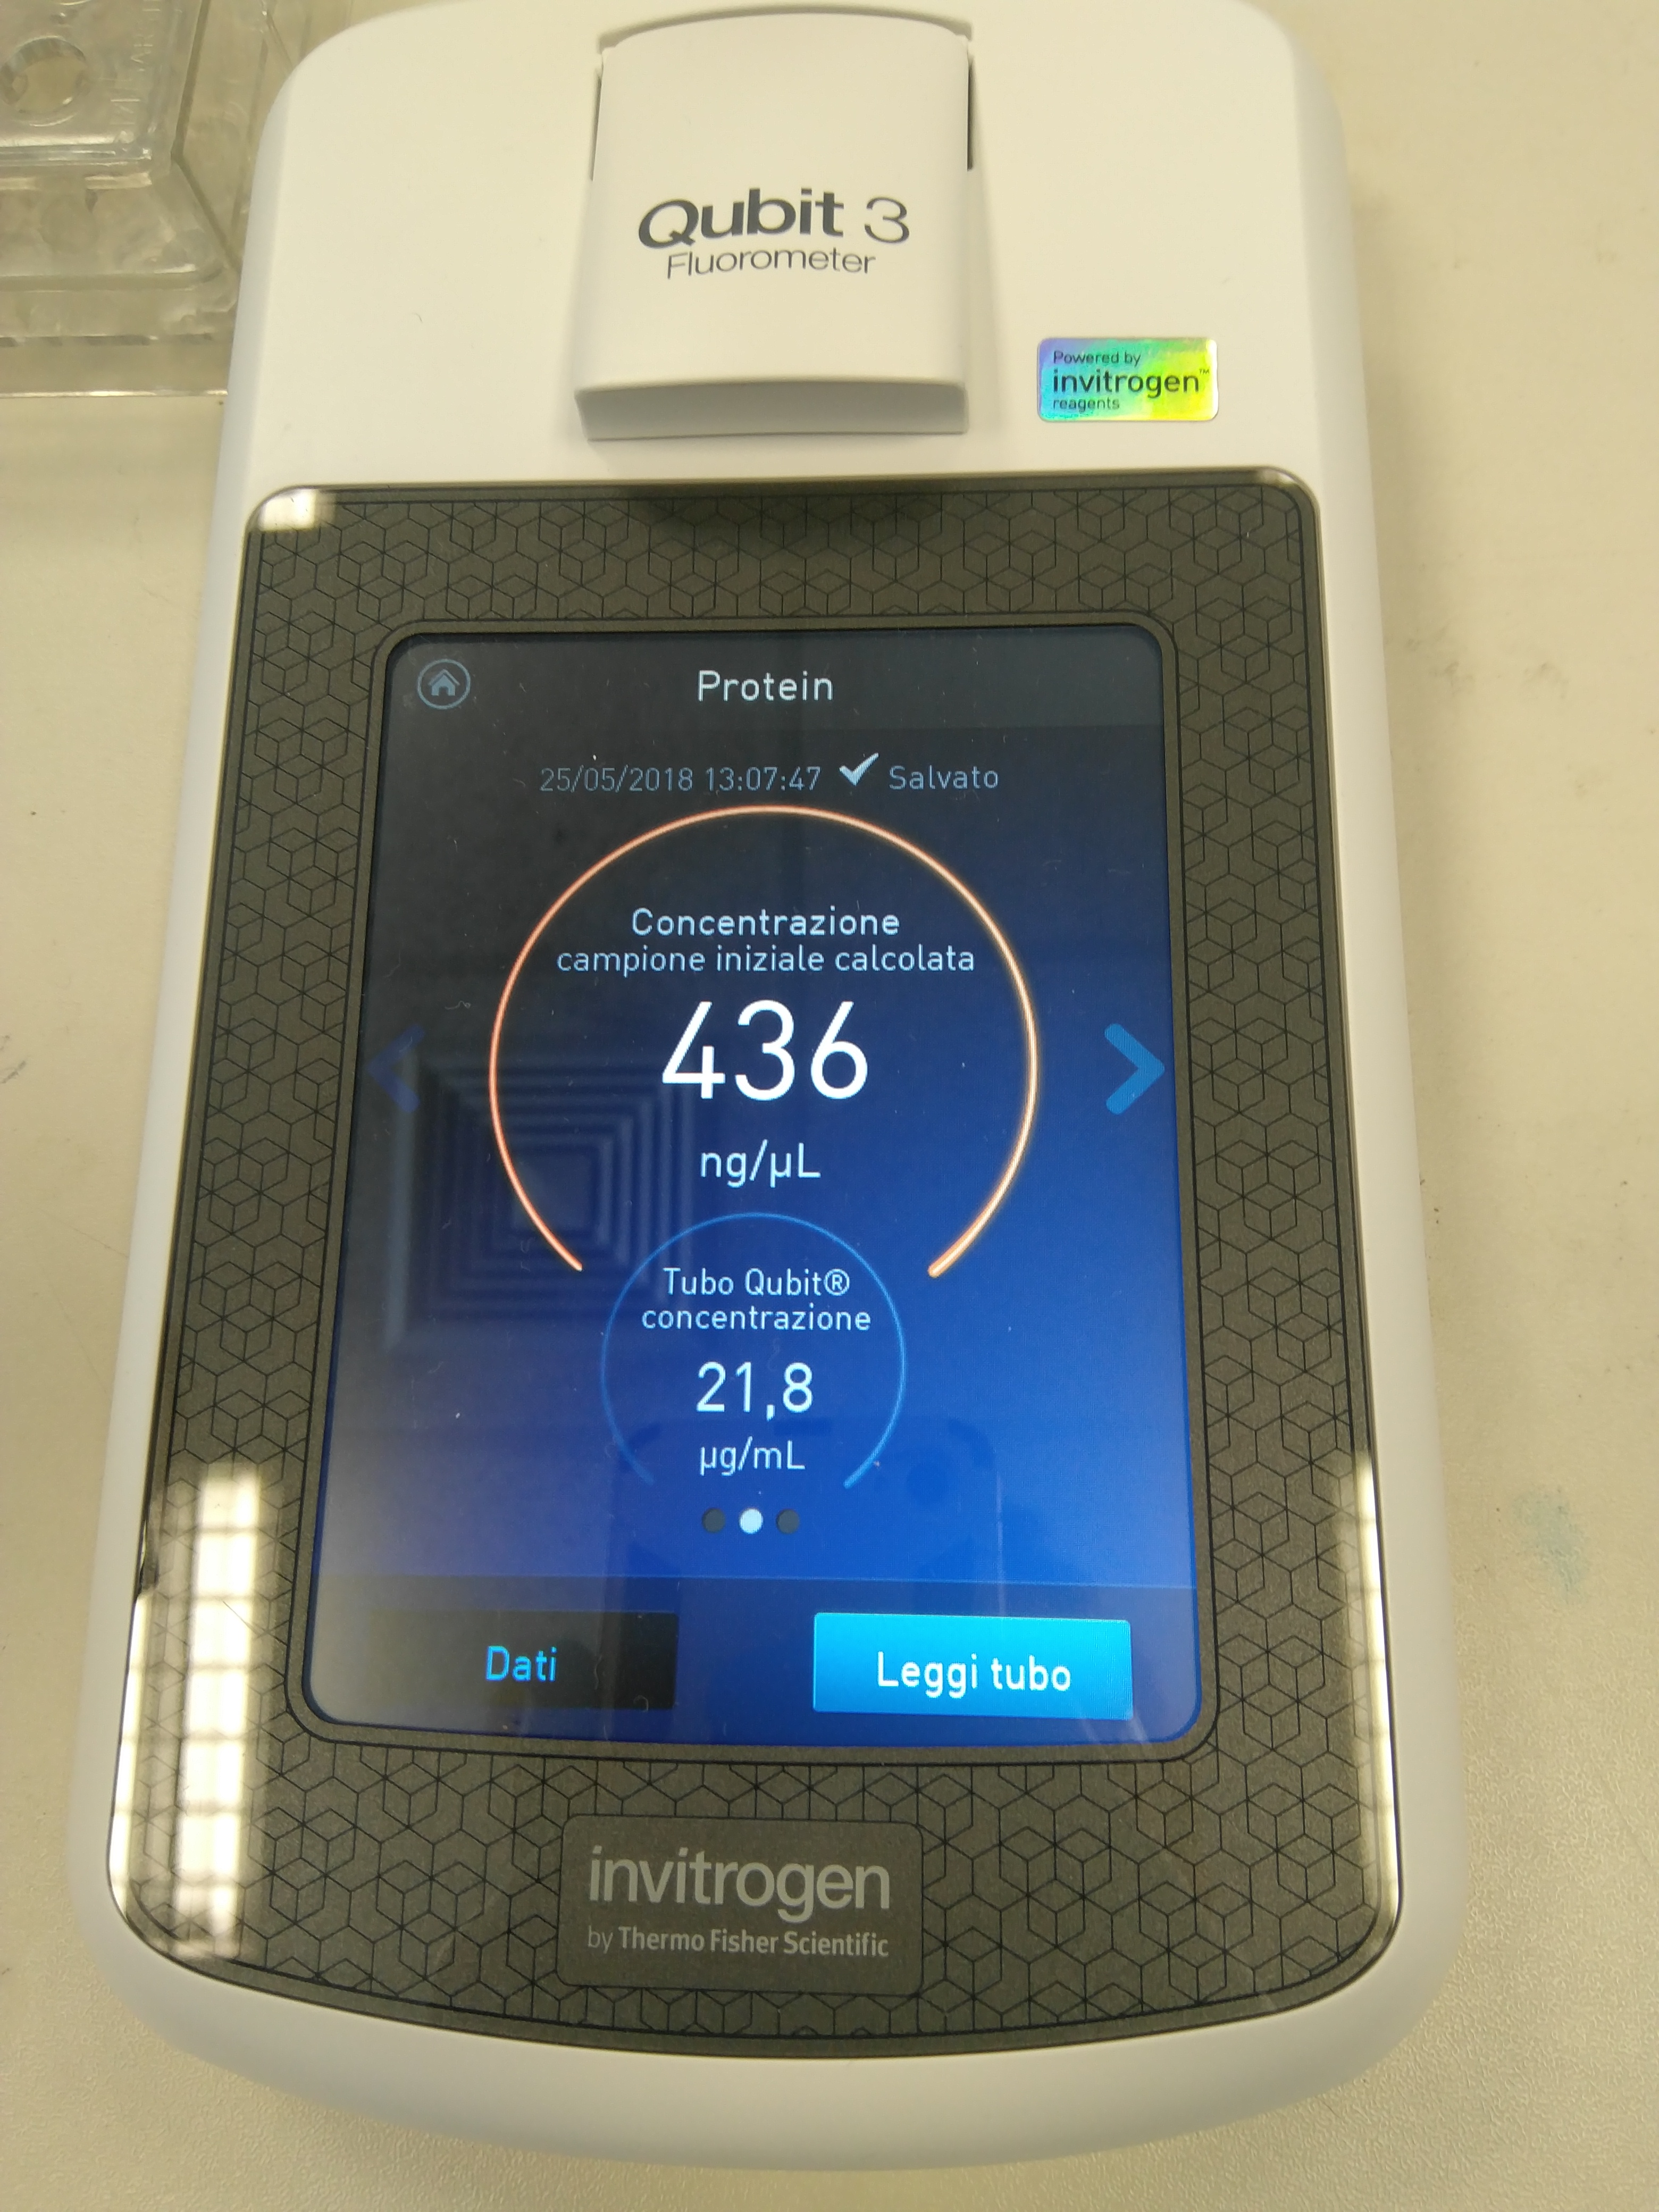
\includegraphics[width=0.4\textwidth]{./immagini/qubit3.jpg}
	\caption{Risultati della quantificazione delle proteine.}
	\label{fig:qubit3}

\end{figure}


\subsection{Risultati e Conclusioni}

\begin{itemize}
\item RealTime PCR:
Come risultato abbiamo osservato un grafico con una curva di amplificazione
con le quantit\`a ad ogni ciclo.
Abbiamo visto che ha un andamento logaritmico.
Tracciando una linea orizzontale e' possibile verificare la soglia di fluorescenza.\\

\item Quantificazione Proteine:
La concentrazione ottenuta per le nostre proteine e' di 436 ng/ul. Visto che eravamo partiti con una
quantita' di 100ul, e 10ul sono stati utilizzati per la quantificazione, moltiplicando per 90ul possiamo
ottenere la quantita' totale di proteine del nostro campione.
\end{itemize}
